\documentclass[10pt,twocolumn]{article}

\usepackage[letterpaper,margin=0.85in,columnsep=0.28in]{geometry}
\usepackage{amsmath,amssymb,amsthm}
\usepackage{bm}
\usepackage{booktabs}
\usepackage{graphicx}
\usepackage{microtype}
\usepackage{caption}
\usepackage[hidelinks]{hyperref}
\usepackage{natbib}
\usepackage{algorithm}
\usepackage{algpseudocode}

\graphicspath{{../figures/}}
\setlength{\emergencystretch}{2.2em}
\captionsetup{font=small,labelfont=bf,skip=5pt}
\setlength{\abovecaptionskip}{5pt}
\setlength{\textfloatsep}{10pt}
\setlength{\dbltextfloatsep}{10pt}
\bibliographystyle{plainnat}
\setlength{\bibsep}{1pt}

\newtheorem{theorem}{Theorem}
\newtheorem{proposition}{Proposition}
\theoremstyle{definition}
\newtheorem{assumption}{Assumption}

\newcommand{\E}{\mathbb{E}}
\newcommand{\Var}{\operatorname{Var}}
\newcommand{\Cov}{\operatorname{Cov}}
\newcommand{\tr}{\operatorname{tr}}
\newcommand{\KL}{\mathrm{KL}}
\newcommand{\R}{\mathbb{R}}
\newcommand{\policy}{\pi_{\theta}}
\newcommand{\score}{\bm{s}}
\newcommand{\ghat}{\hat{\bm{g}}}
\newcommand{\gbar}{\bar{\bm{g}}}
\newcommand{\Sb}{\Sigma_{\mathrm{b}}}
\newcommand{\Sw}{\Sigma_{\mathrm{w}}}
\newcommand{\Bcrit}{B_{\mathrm{crit}}}

\newcommand{\numAbstainLarge}{160.5}
\newcommand{\numAbstainLargeChecks}{4}
\newcommand{\numAbstainLargeLive}{3}
\newcommand{\numAbstainSmall}{2.0}
\newcommand{\numAbstainSmallChecks}{4}
\newcommand{\numAbstainSmallLive}{2}
\newcommand{\numAdamScaleBase}{0.203}
\newcommand{\numAdamScaleBinomial}{0.0051}
\newcommand{\numAdamScaleForecast}{0.0207}
\newcommand{\numAdamScaleHalfHigh}{0.0287}
\newcommand{\numAdamScaleHalfLow}{0.0052}
\newcommand{\numAdamScaleHalfRatio}{5.5}
\newcommand{\numAdamScaleMean}{0.362}
\newcommand{\numAdamScaleResolved}{0.0892}
\newcommand{\numAdamScaleResolvedHigh}{0.1193}
\newcommand{\numAdamScaleResolvedLow}{0.0398}
\newcommand{\numAdamScaleSeeds}{10}
\newcommand{\numAdamScaleShortfall}{4.3}
\newcommand{\numAdamScaleShortfallHigh}{17}
\newcommand{\numAdamScaleShortfallLow}{3.1}
\newcommand{\numAdamScaleSpread}{0.0893}
\newcommand{\numAdamScaleStateGain}{8.7}
\newcommand{\numAdamScaleStateless}{0.00237}
\newcommand{\numAdamScaleStatelessShortfall}{38}
\newcommand{\numAdamScaleWidePrompts}{32}
\newcommand{\numDiagAurocHigh}{0.74}
\newcommand{\numDiagAurocLow}{0.68}
\newcommand{\numDiagCells}{192}
\newcommand{\numDiagCoverage}{80}
\newcommand{\numDiagFailsHigh}{16}
\newcommand{\numDiagFailsLow}{34}
\newcommand{\numDiagHigh}{0.0488}
\newcommand{\numDiagLow}{0.0044}
\newcommand{\numDiagOtherEnvAurocHigh}{0.87}
\newcommand{\numDiagOtherEnvAurocLow}{0.71}
\newcommand{\numDiagOtherEnvCells}{96}
\newcommand{\numDiagOtherEnvCoverage}{82}
\newcommand{\numDiagOtherEnvFailsHigh}{3}
\newcommand{\numDiagOtherEnvFailsLow}{5}
\newcommand{\numDiagOtherEnvHigh}{0.0507}
\newcommand{\numDiagOtherEnvLow}{0.0044}
\newcommand{\numDiagOtherEnvRank}{0.07}
\newcommand{\numDiagOtherEnvThreshold}{0.0300}
\newcommand{\numDiagOtherEnvWorstAll}{2.13}
\newcommand{\numDiagOtherEnvWorstKept}{1.58}
\newcommand{\numDiagOtherEnvWorstPercentile}{91}
\newcommand{\numDiagRank}{0.26}
\newcommand{\numDiagReplicateAurocHigh}{0.87}
\newcommand{\numDiagReplicateAurocLow}{0.79}
\newcommand{\numDiagReplicateCells}{192}
\newcommand{\numDiagReplicateCoverage}{78}
\newcommand{\numDiagReplicateFailsHigh}{16}
\newcommand{\numDiagReplicateFailsLow}{36}
\newcommand{\numDiagReplicateHigh}{0.0479}
\newcommand{\numDiagReplicateLow}{0.0046}
\newcommand{\numDiagReplicateRank}{0.26}
\newcommand{\numDiagReplicateThreshold}{0.0300}
\newcommand{\numDiagReplicateWorstAll}{1.48}
\newcommand{\numDiagReplicateWorstKept}{1.48}
\newcommand{\numDiagReplicateWorstPercentile}{64}
\newcommand{\numDiagThreshold}{0.0300}
\newcommand{\numDiagWorstAll}{1.58}
\newcommand{\numDiagWorstKept}{1.58}
\newcommand{\numDiagWorstPercentile}{62}
\newcommand{\numEarlyCorrelation}{+0.31}
\newcommand{\numEarlyCorrelationBig}{+0.11}
\newcommand{\numEarlyCorrelationHigh}{+0.73}
\newcommand{\numEarlyCorrelationLow}{-0.27}
\newcommand{\numFirstHalfShare}{55}
\newcommand{\numForecastHeadlinePool}{24}
\newcommand{\numForecastInside}{162}
\newcommand{\numForecastMedian}{1.11}
\newcommand{\numForecastReplicateInside}{158}
\newcommand{\numForecastReplicateMedian}{1.10}
\newcommand{\numForecastReplicatePool}{16}
\newcommand{\numForecastReplicateWorst}{1.48}
\newcommand{\numForecastSeeds}{48}
\newcommand{\numForecastSettings}{192}
\newcommand{\numForecastSpreadRange}{47}
\newcommand{\numForecastWorst}{1.58}
\newcommand{\numLateCorrelation}{+0.18}
\newcommand{\numMemoryFraction}{1.00}
\newcommand{\numMemorySettings}{288}
\newcommand{\numMixedBase}{0.257}
\newcommand{\numMixedDecision}{accept}
\newcommand{\numMixedForecast}{0.0660}
\newcommand{\numMixedHalfRatio}{1.56}
\newcommand{\numMixedLive}{0.45}
\newcommand{\numMixedMean}{0.517}
\newcommand{\numMixedObserved}{0.0485}
\newcommand{\numMixedRatio}{1.4}
\newcommand{\numMixedResidual}{3.1}
\newcommand{\numMixedResolved}{0.0480}
\newcommand{\numMixedResolvedHigh}{0.0560}
\newcommand{\numMixedResolvedLow}{0.0338}
\newcommand{\numMixedSeeds}{16}
\newcommand{\numNullCoin}{90.5}
\newcommand{\numNullGap}{671}
\newcommand{\numNullLearning}{0.14}
\newcommand{\numNullPassEnd}{0.90}
\newcommand{\numNullPassStart}{0.31}
\newcommand{\numNullUpdates}{80}
\newcommand{\numPickAdjoint}{75}
\newcommand{\numPickAdjointLow}{63}
\newcommand{\numPickConstant}{66}
\newcommand{\numPickFrozen}{74}
\newcommand{\numPickGain}{8.8}
\newcommand{\numPickGainHi}{15.6}
\newcommand{\numPickGainLo}{1.7}
\newcommand{\numPickOracle}{77}
\newcommand{\numPickOraclePoints}{10.2}
\newcommand{\numPickShare}{0.86}
\newcommand{\numPickTasks}{12}
\newcommand{\numPropagatedMedian}{1.03}
\newcommand{\numPropagatedPercent}{3}
\newcommand{\numPropagatedWorst}{1.2}
\newcommand{\numPropagationSettings}{54}
\newcommand{\numRealFirstHalfShare}{5}
\newcommand{\numRealSizeAdjoint}{8.95}
\newcommand{\numRealSizeAllPairs}{15}
\newcommand{\numRealSizeConstantGain}{1.10}
\newcommand{\numRealSizeEmpiricalGain}{0.95}
\newcommand{\numRealSizeEmpiricalHi}{1.15}
\newcommand{\numRealSizeEmpiricalLo}{0.85}
\newcommand{\numRealSizeError}{1.61}
\newcommand{\numRealSizeErrorWorst}{2.75}
\newcommand{\numRealSizeFixed}{12.53}
\newcommand{\numRealSizeFixedGain}{1.41}
\newcommand{\numRealSizeFixedHi}{1.65}
\newcommand{\numRealSizeFixedLo}{1.28}
\newcommand{\numRealSizeMargin}{2}
\newcommand{\numRealSizeOracleGain}{1.05}
\newcommand{\numRealSizeOracleHi}{1.19}
\newcommand{\numRealSizeOracleLo}{0.95}
\newcommand{\numRealSizePairs}{4}
\newcommand{\numRealSizeRecipes}{6}
\newcommand{\numRealSizeRuns}{102}
\newcommand{\numRealSizeSeeds}{16}
\newcommand{\numRealSizeTarget}{1}
\newcommand{\numRolloutShareGeight}{65}
\newcommand{\numRolloutShareGfour}{82}
\newcommand{\numRolloutShareGsixteen}{46}
\newcommand{\numRolloutShareGtwo}{93}
\newcommand{\numRolloutShareMedian}{78}
\newcommand{\numSatDegenerate}{100}
\newcommand{\numSatDisagreeing}{0}
\newcommand{\numSatKLhigh}{7.7e-2}
\newcommand{\numSatKLlow}{1.8e-5}
\newcommand{\numSatPrompts}{32}
\newcommand{\numSatScore}{0.875}
\newcommand{\numScalarMedian}{57.93}
\newcommand{\numScalarWorst}{791.5}
\newcommand{\numScaleBase}{0.203}
\newcommand{\numScaleDivergenceEnd}{5.47}
\newcommand{\numScaleDivergenceStart}{0.37}
\newcommand{\numScaleFullSlope}{+0.96}
\newcommand{\numScaleGain}{0.110}
\newcommand{\numScaleHigh}{0.460}
\newcommand{\numScaleLow}{0.208}
\newcommand{\numScaleMean}{0.313}
\newcommand{\numScaleRuns}{8}
\newcommand{\numScaleShare}{84}
\newcommand{\numScaleSpread}{0.0925}
\newcommand{\numScaleTailSlope}{+0.09}
\newcommand{\numScanCliffHigh}{0.990}
\newcommand{\numScanCliffLow}{0.000}
\newcommand{\numScanFamilies}{24}
\newcommand{\numScanLargeUsable}{7}
\newcommand{\numScanMatched}{18}
\newcommand{\numScanSmallUsable}{24}
\newcommand{\numSizeAdjointRuns}{3.07}
\newcommand{\numSizeArms}{192}
\newcommand{\numSizeCap}{16}
\newcommand{\numSizeConstantGain}{1.93}
\newcommand{\numSizeConstantHi}{2.28}
\newcommand{\numSizeConstantLo}{1.45}
\newcommand{\numSizeEmpiricalGain}{2.13}
\newcommand{\numSizeEmpiricalHi}{2.38}
\newcommand{\numSizeEmpiricalLo}{1.98}
\newcommand{\numSizeEmpiricalRuns}{6.52}
\newcommand{\numSizeFixedGain}{9.57}
\newcommand{\numSizeFixedHi}{10.56}
\newcommand{\numSizeFixedLo}{7.24}
\newcommand{\numSizeFixedRuns}{30.4}
\newcommand{\numSizeForecastError}{1.11}
\newcommand{\numSizeFrozenGain}{1.09}
\newcommand{\numSizeFrozenRelative}{1.26}
\newcommand{\numSizeFrozenRelativeWorst}{2.43}
\newcommand{\numSizeFrozenRuns}{3.34}
\newcommand{\numSizeFrozenScale}{84}
\newcommand{\numSizeFrozenScaleSpread}{4.8}
\newcommand{\numSizeFrozenVsFixed}{9.1}
\newcommand{\numSizeHoldout}{32}
\newcommand{\numSizeOracleGain}{1.02}
\newcommand{\numSizeOracleHi}{1.05}
\newcommand{\numSizeOracleLo}{0.99}
\newcommand{\numSizeOracleRuns}{3.16}
\newcommand{\numSizeOverlapEmpirical}{1.65}
\newcommand{\numSizeOverlapFixed}{4.76}
\newcommand{\numSizeOverlapRuns}{2.85}
\newcommand{\numSizePairs}{1020}
\newcommand{\numSizeSeeds}{48}
\newcommand{\numSizeTarget}{0.1}
\newcommand{\numSpectrumFastest}{0.979}
\newcommand{\numSpectrumRadiusMax}{1.0199}
\newcommand{\numSpectrumRadiusMin}{1.0001}
\newcommand{\numSpectrumShareHigh}{51}
\newcommand{\numSpectrumShareLow}{31}
\newcommand{\numSweepBands}{4}
\newcommand{\numSweepBest}{1.24}
\newcommand{\numSweepErrors}{1.66, 2.13, 2.80, 1.24}
\newcommand{\numSweepHalfHigh}{1.30}
\newcommand{\numSweepHalfLow}{1.01}
\newcommand{\numSweepInside}{1}
\newcommand{\numSweepWinBand}{0.85}
\newcommand{\numSweepWinForecast}{0.0205}
\newcommand{\numSweepWinGain}{0.275}
\newcommand{\numSweepWinHigh}{0.0337}
\newcommand{\numSweepWinLow}{0.0105}
\newcommand{\numSweepWinMeasured}{0.0253}
\newcommand{\numSweepWinRatio}{1.24}
\newcommand{\numSweepWinResidual}{8.0}
\newcommand{\numSweepWorst}{2.80}
\newcommand{\numTiltedEarly}{254}
\newcommand{\numTolClean}{3.07}
\newcommand{\numTolFixed}{30.4}
\newcommand{\numTolLooseBreakeven}{4.2}
\newcommand{\numTolLooseClean}{2.22}
\newcommand{\numTolLooseFixed}{5.61}
\newcommand{\numTolLooseTarget}{1}
\newcommand{\numTolRunsDouble}{9.5}
\newcommand{\numTolRunsOneHalf}{5.4}
\newcommand{\numTolRunsQuadruple}{18.7}
\newcommand{\numTolRunsTwoHalf}{13.3}
\newcommand{\numTolScaleRange}{100}
\newcommand{\numTolScaleSpread}{1.000}
\newcommand{\numTolTarget}{0.1}
\newcommand{\numTolTested}{12}
\newcommand{\numTraceRuns}{10}
\newcommand{\numTraceWindow}{3}
\newcommand{\numWalkMedian}{1.06}
\newcommand{\numWalkWorst}{3.8}

\newcommand{\ruledtitle}[1]{%
  \par\noindent\rule{\textwidth}{1.6pt}\par\vspace{3pt}
  {\centering\fontsize{15}{17}\selectfont\bfseries #1\par}
  \vspace{3pt}\noindent\rule{\textwidth}{0.4pt}\par
}

\begin{document}

\twocolumn[
  \ruledtitle{How Many Runs Does an RL Post-Training Comparison Need?\\
  Forecasting Run-to-Run Spread from a Single Run}
  \vspace{6pt}
  {\centering
    \normalsize Mehmet Demir G\"uven$^{\dagger}$\par\vspace{2pt}
    \normalsize\textbf{ETH Z\"urich}$^{*}$\par\vspace{1pt}
    \small\texttt{dgueven@student.ethz.ch}\par
  }
  \vspace{6pt}
  \begin{minipage}{\textwidth}
  \begin{center}\textbf{Abstract}\end{center}
  \vspace{-4pt}
  \begin{quote}
  Reinforcement learning post-training is compared from single runs, and how many runs a
  comparison needs is set by a quantity nobody measures: how much a rerun would move the score.
  The usual recourse is to fix the run count in advance, or to spend runs estimating the spread
  before the comparison can begin, because after one run per arm there is no empirical spread to
  put in a stopping rule.

  We forecast it instead. Training noise is not accumulated: a perturbation entering at one update
  is reweighted by every update that follows, so the covariance of a run about its mean obeys
  $S_{t+1} = A_t S_t A_t^{\!\top} + Q_t$. Carrying the gradient of the reported metric backwards
  along one stored trajectory turns that recursion into the across-seed variance of the metric, as
  a sum of scalars with no covariance matrix formed. Frozen before the remaining seeds existed, it
  has a median error of $\numForecastMedian\times$ over $\numForecastSettings$ settings.

  Used to size comparisons, it matches a rule told the realised spread
  ($\numSizeOracleGain\times$ {$[\numSizeOracleLo, \numSizeOracleHi]$}) and needs
  $\numSizeFixedGain\times$ {$[\numSizeFixedLo, \numSizeFixedHi]$} fewer runs than fixed-budget
  practice across $\numSizePairs$ comparisons, graded on seeds no policy may see. Corrupting the
  forecast on purpose shows a systematic scale error is free, since the stopping threshold absorbs
  it, and that the procedure pays until relative error reaches about $\numTolBreakeven\times$.

  On pretrained models accuracy is regime-dependent. Across $\numSweepBands$ pre-specified regimes
  on Qwen2.5-0.5B the frozen forecast misses by factors of $\numSweepErrors$, all of them inside
  that break-even, while a corpus whose reward groups go unanimous carries no seed noise to
  forecast and misses by twenty-five. We report the break-even rather than the method alone.
  \end{quote}
  \end{minipage}
  \vspace{6pt}

  \begin{minipage}{\textwidth}
    \scriptsize
    \noindent\rule{0.32\columnwidth}{0.4pt}\par\vspace{2pt}
    \noindent $^{*}$Department of Computer Science, ETH Z\"urich, 8092 Zurich, Switzerland.

    \smallskip
    \noindent $^{\dagger}$ETH Z\"urich neither endorsed, supervised nor funded this work; the author was enrolled as an undergrad at the programme BSc Computer Science during this research, hence the affiliation.
  \end{minipage}
  \vspace{4pt}
]



\section{Introduction}
\label{sec:introduction}

Reinforcement learning with verifiable rewards is the standard way to turn a pretrained model into
a reasoning one \citep{deepseekr1}, and a paper reports that a recipe moved a benchmark by two
points. Whether that is a result depends on a number nobody has: how much the same recipe would
have moved it under a different seed. The problem is documented
\citep{henderson2018matters, hochlehnert2025sober}, and the only instrument the field has for it is
replication, which at RL post-training cost is close to unaffordable.

The practical form of the problem is not reporting but budgeting. Deciding that one recipe beats
another means training seeds of each until the lead is convincing, and how many that takes is
governed by the across-seed deviation. A practitioner who does not have it either fixes the seed
count in advance, or spends seeds estimating it before the comparison can start. Both are
expensive, and the second is expensive for a structural reason: after a single run per arm there is
no empirical deviation at all, so the first two runs of every arm buy no evidence about the
question being asked.

This paper forecasts that deviation from one run, and then spends it. The route runs through a
correction to the obvious model of where run-to-run spread comes from. That model says gradient
noise perturbs each update, perturbations accumulate, two runs execute a random walk away from each
other, and reproducibility decays with run length. It is wrong. Noise from one update does not
survive to the end of training unchanged: it is passed through every update that follows, which
reweights it. What reaches the end is a convolution of injected noise with the sensitivity of the
remaining trajectory, an object that obeys a recursion and that can be carried against the gradient
of the reported metric rather than being formed.

\paragraph{Contributions.}
\begin{itemize}\itemsep2pt
  \item \textbf{An error bar from one run} (Theorem~\ref{thm:adjoint}). Carrying the metric
  gradient backwards along a single stored trajectory gives the across-seed variance of the
  reported score as a sum of scalars, one per update, with no covariance matrix formed. The
  transpose a backward pass would need is free, because the mean update of any count-based
  estimator is the gradient of a scalar potential and its Jacobian is therefore symmetric. Frozen
  before the remaining seeds were trained, its median error is $\numForecastMedian\times$ across
  $\numForecastSettings$ settings.

  \item \textbf{Comparisons sized from one run} (Section~\ref{sec:sizing}). Supplying the deviation
  from the first run of each arm settles $\numSizePairs$ comparisons at a $\numSizeTarget\%$
  mistake rate in $\numSizeAdjointRuns$ runs, indistinguishable from the $\numSizeOracleRuns$ of a
  rule handed the realised deviation, against $\numSizeFixedRuns$ for fixed-budget practice: a
  saving of $\numSizeFixedGain\times$ {$[\numSizeFixedLo, \numSizeFixedHi]$}, graded against an
  ordering fixed on seeds no policy may draw. Estimating the deviation from spent seeds instead
  costs $\numSizeEmpiricalGain\times$, most of it structural.

  \item \textbf{The condition under which it pays.} Corrupting the forecast deliberately puts the
  break-even against a fixed budget at $\numTolLooseBreakeven\times$ relative error, and shows
  that a systematic scale error costs nothing at all across
  $\numTolScaleRange$ orders of magnitude, because the stopping threshold absorbs it. A forecast
  used this way does not need to be calibrated, which is the opposite of what reporting an error
  bar requires.

  \item \textbf{An honest boundary} (Section~\ref{sec:real}). On Qwen2.5-0.5B accuracy is
  regime-dependent: across $\numSweepBands$ pre-specified regimes the errors are
  $\numSweepErrors$, all inside the break-even above, while a corpus whose reward groups go
  unanimous injects no seed noise and is missed by twenty-five. At $7$B under Adam the forecast is
  short by between $\numAdamScaleShortfallLow$ and $\numAdamScaleShortfallHigh$.
\end{itemize}

Every experiment here runs on one laptop, which bounds what any of it establishes about
frontier-scale RLVR and is stated plainly in Section~\ref{sec:discussion}.

\section{Setup}
\label{sec:setup}

A policy $\policy(y \mid x)$ answers a prompt $x \sim \mathcal{D}$ and a verifier returns a binary
reward $r(x,y) \in \{0,1\}$. The objective is $J(\theta) = \E_x[p(x)]$ with
$p(x) := \Pr[r = 1 \mid x]$. Write $\score(y) := \nabla_\theta \log \policy(y \mid x)$, so
$\E_y[\score] = 0$, and let $u_r := \E[\score \mid r]$. Because the reward is binary, every
quantity below depends on the policy only through the per-prompt objects $(p, u_1, S_0, S_1)$,
where $S_r := \Cov(\score \mid r)$, which is what makes an exact finite-$G$ treatment possible.

A batch is $P$ prompts drawn from $\mathcal{D}$ with $G$ responses each; $R = PG$ is fixed by
hardware. With $k$ the number of successes in a group we consider any advantage of the form
$A_j = w(k, r_j)$, which covers RLOO \citep{ahmadian2024rloo}, GRPO with a mean baseline
\citep{liu2025drgrpo}, standardised GRPO \citep{shao2024deepseekmath} and a fixed external
baseline. The per-prompt and batch estimators are
$z := G^{-1}\sum_j w(k, r_j)\score(y_j)$ and $\ghat := P^{-1}\sum_i z_i$.

\paragraph{Two levels of noise.} Prompts are sampled and then responses are sampled within each
prompt, so by the law of total variance
\begin{equation}
  \label{eq:two-level}
  \Cov(\ghat) \;=\; \frac{1}{P}\Big[\, \Sb + \tfrac{1}{G-1}\Sw \,\Big],
\end{equation}
with $\Sb$ the covariance across prompts of the per-prompt mean update and $\Sw$ the within-prompt
term, written in the $(G-1)$ convention the leave-one-out estimators use. Both traces are
recoverable from the microbatch gradients a trainer already accumulates. We write
$\tau_{\mathrm{b}}$ and $\tau_{\mathrm{w}}$ for those traces.

\paragraph{Intervals.} Seed experiments produce pairwise quantities: $n$ runs give $\binom{n}{2}$
distances, which are not $\binom{n}{2}$ observations, since every run appears in $n-1$ of them.
Treating them as independent understates the standard error by roughly a factor of two at the seed
counts anyone trains. Every interval here resamples \emph{runs} and rebuilds the pairwise quantity
from the resampled set.

\section{Noise is filtered, not accumulated}
\label{sec:theory}

Fix a policy $\theta_0$ and start two runs from it. They share parameters, optimiser state, data
distribution and recipe, and independently draw everything the seed controls: which prompts each
batch contains and which responses are sampled. That is the comparison a practitioner makes when
they rerun, and it is the estimand throughout, so both terms of \eqref{eq:two-level} contribute.

Write $\delta_t := \theta_t - \bar\theta_t$ for one run's departure from the mean trajectory. With
updates $\theta \leftarrow \theta + \eta\ghat$ and
$\mathcal{J}_t := \partial\gbar/\partial\theta$,
\begin{equation}
  \label{eq:seed-recursion}
  \delta_{t+1} = A_t \delta_t + \eta\,\xi_t,
  \qquad A_t := I + \eta \mathcal{J}_t,
\end{equation}
to first order in $\delta$, where $\E[\xi_t \mid \mathcal{F}_t] = 0$ and
$\Cov(\xi_t) = \Sigma_t/P$.

If the objective were flat, $\mathcal{J} = 0$, this would be a random walk: divergence would
accumulate as $\E\|\Delta_t\|^2 \propto t$ and a longer run would be strictly less reproducible.
That is the implicit model behind measuring run-to-run variance by brute force. But two RLVR runs
climb the same objective, and $A_t$ reweights a perturbation rather than passing it through.

\begin{theorem}[Finite-time covariance]
  \label{thm:propagation}
  Let $S_t := \Cov(\delta_t)$, with $S_0 = 0$ when runs start together. Under
  \eqref{eq:seed-recursion},
  \begin{equation}
    \label{eq:lyapunov}
    S_{t+1} = A_t S_t A_t^{\!\top} + Q_t,
    \qquad Q_t := \eta^2 \Sigma_t / P,
  \end{equation}
  hence $S_T = \sum_{t<T} \Phi_{T,t+1} Q_t \Phi_{T,t+1}^{\!\top}$ with
  $\Phi_{T,s} := \prod_{u=s}^{T-1} A_u$ taken in order of decreasing $u$. Two independent seeds
  satisfy $\Cov(\theta^A_T - \theta^B_T) = 2S_T$.
\end{theorem}

\begin{proof}[Proof sketch]
  Taking the covariance of \eqref{eq:seed-recursion} leaves a cross term
  $\E[\delta_t \xi_t^{\!\top}]$. It vanishes without assuming $\xi_t$ and $\delta_t$ are
  independent, which they are not, since the batch noise is drawn at $\theta_t$ and that parameter
  was produced by earlier noise. What holds is that $\xi_t$ is a martingale difference,
  $\E[\xi_t \mid \mathcal{F}_t] = 0$, and $\delta_t$ is $\mathcal{F}_t$-measurable, so the cross
  term is zero by the tower rule. Unrolling from $S_0 = 0$ gives the sum.
\end{proof}

The factor of two belongs to the difference of two runs and not to the covariance of one; keeping
them apart is what makes the statement unambiguous.

\subsection{Carrying it to the number that gets reported}

Equation \eqref{eq:lyapunov} concerns policies. What a paper reports is a score $M(\theta)$:
pass rate, exact match, win rate. Linearising about the endpoint,
$\Var_{\text{seed}}[M(\theta_T)] \approx \nabla M^{\!\top} S_T \nabla M$, which needs a matrix
nobody can form for a real model. It is not needed.

\begin{theorem}[Adjoint form of the reported spread]
  \label{thm:adjoint}
  Define $b_T := \nabla M(\theta_T)$ and $b_s := A_s^{\!\top} b_{s+1}$ for $s = T-1,\dots,0$. Then
  \begin{equation}
    \label{eq:adjoint}
      V^{\text{lin}}_T \,=\, \sum_{t=0}^{T-1} b_{t+1}^{\!\top} Q_t\, b_{t+1}
      \,=\, \frac{\eta^2}{P}\sum_{t=0}^{T-1} \Var_{i}\!\big(b_{t+1}^{\!\top} z_{t,i}\big),
  \end{equation}
  the variance taken over prompts.
\end{theorem}

\begin{proof}[Proof sketch]
  $b_s = \Phi_{T,s}^{\!\top}\nabla M$ by induction; substitute the unrolled $S_T$. The second
  equality is $Q_t = \eta^2\Sigma_t/P$ with
  $b^{\!\top}\Sigma_t b = \Var_i(b^{\!\top} z_{t,i})$, since $\Sigma_t$ is the covariance of one
  prompt's contribution rather than of the batch mean.
\end{proof}

The equality is exact for $V^{\text{lin}}_T$, the variance of the metric linearised at
$\bar\theta_T$. The quantity a practitioner wants is $\Var_{\text{seed}}[M(\theta_T)]$, and the two
agree to the order at which the linearisation holds; Section~\ref{sec:real} is about when that
agreement fails. Every term of \eqref{eq:adjoint} is one scalar per update, which a trainer can
accumulate alongside the update it is already making.

What the backward pass costs depends on $A_s^{\!\top}$, and here the estimator family pays for
itself.

\begin{proposition}[The mean update is a gradient field]
  \label{prop:potential}
  For any count-based estimator, $\gbar(\theta) = \nabla_\theta\,\Psi(\theta)$ with
  $\Psi(\theta) = \E_x[\Lambda(p_x)]$ and $\Lambda' = \lambda$, where the per-prompt mean update is
  $\lambda(p_x, G)\nabla_\theta p_x$. Hence $\mathcal{J} = \nabla^2\Psi$ is symmetric and
  $A_s^{\!\top} = A_s$.
\end{proposition}

Because $\lambda$ depends on $\theta$ only through $p_x$, $\lambda(p_x)\nabla p_x = \nabla
\Lambda(p_x)$, and averaging over $x$ commutes with the gradient. We call $\Psi$ the
\emph{estimator potential}; it is not the objective $J$ unless $\lambda \equiv 1$, and the gap is
exactly the difficulty reweighting the estimator applies. For RLOO the potential is the pass rate
itself. The practical consequence is that the backward pass needs no transpose and can be run with
the same code path as the forward one.

\subsection{Linearising the model instead of the run}
\label{sec:tangent}

Theorem~\ref{thm:adjoint} is exact in the model and first-order in the distance between runs, and
it inherits its one run's blind spot: at a run that has saturated, $\nabla M(\theta_T) = 0$ and the
forecast vanishes, wherever the other seeds went. The opposite linearisation is available. With
$\score_0(x,y) := \nabla_\theta\log\pi_{\theta_0}(y \mid x)$ the score at the starting parameters,
the \emph{tangent policy}
\begin{equation}
  \label{eq:tangent}
  \pi'_{\vartheta}(y \mid x) \;\propto\;
  \pi_{\theta_0}(y \mid x)\,\exp\!\big(\score_0(x,y)^{\!\top}\vartheta\big)
\end{equation}
is an exponential family in the frozen scores. Updating $\vartheta$ with an estimator of
\eqref{eq:family} needs sampled responses, their rewards and inner products of frozen scores, and
no pass through the model, so seeds can be \emph{simulated} by the thousand with the sampling, the
estimator's weights and the saturation all kept exactly.

\begin{proposition}[When a simulated seed is a real one]
  \label{prop:tangent}
  If $\log\policy(y \mid x)$ is affine in $\theta$ up to a per-prompt normaliser, the run from
  $\theta_0$ and the tangent run from $\vartheta_0 = 0$ have the same law, so $M(\theta_T)$ has the
  distribution of its simulated counterpart.
\end{proposition}

Both are then Markov chains with one transition kernel. A softmax over one decision qualifies. A
network does not: there a simulated run is exact in its first update and drifts as the scores
move. This is the tangent-kernel approximation \citep{jacot2018ntk, malladi2023kernel}, used to
draw many runs instead of predicting one.

\section{Running it}
\label{sec:estimation}

\begin{algorithm}[t]
\caption{The forecast, as a trainer would run it}
\label{alg:forecast}
\small
\begin{algorithmic}[1]
  \State train as usual, storing $\theta_t$ and $\eta_t$ for each update
  \State $b \gets \nabla M(\theta_T)$ \Comment{one rollout and backward pass on the eval set}
  \State $v \gets 0$
  \For{$t = T-1$ \textbf{down to} $0$}
    \State draw a batch at $\theta_t$; let $\hat{g}_{t,i}$ be its per-prompt gradients
    \State $v \gets v + (\eta_t^2/P)\,\widehat{\Var}_i\big(b^{\!\top}\hat{g}_{t,i}\big)$
      \Comment{one scalar}
    \If{transport is needed}
      \State $\delta \gets \epsilon\, b/\|b\|$
      \State $b \gets b + \dfrac{\eta_t}{2}\cdot\dfrac{\|b\|}{\epsilon}
        \big(\gbar(\theta_t + \delta) - \gbar(\theta_t - \delta)\big)$
        \Comment{common random numbers}
    \EndIf
  \EndFor
  \State \Return $\sqrt{v}$
\end{algorithmic}
\end{algorithm}

\paragraph{What it costs, plainly.} As written, the backward pass makes three passes per stored
update: one batch for the injected term and two for the Hessian-vector product. That is about three
times the compute of the training run, not a rounding error, and we would rather state it than let
a reader discover it.

It is also usually unnecessary. Ablating the transport, holding $b$ at $\nabla M(\theta_T)$ instead
of carrying it back, changes the forecast by a median of $2\%$ and the median error not at all over
runs of ten and twenty-five updates. The reason is in the spectrum of $A_t$: most of it sits within
$10^{-4}$ of one and $\nabla M$ points into that part, so $\Phi_{T,t}$ is close to the identity
along the one direction the forecast needs. What we recommend is the cheap estimator,
\begin{equation}
  \label{eq:cheap}
  \Var_{\text{seed}}\big[M(\theta_T)\big] \;\approx\;
  \sum_{t} \frac{\eta_t^2}{P}\,\widehat{\Var}_i\!\big(\nabla M(\theta_T)^{\!\top}\hat{g}_{t,i}\big),
\end{equation}
one extra pass per update and no Hessian-vector products, with the full recursion held in reserve
for runs long enough, or curvature strong enough, that a per-update discrepancy of a percent
compounds. Knowing which regime one is in is what the recursion is for.

\paragraph{A closed form with no run at all.} Take \eqref{eq:cheap} with $\Phi \approx I$ and a
constant step, replace the projection $\Var_i(\nabla M^{\!\top}\hat g_{t,i})$ by the trace
\eqref{eq:two-level}, and the run drops out entirely:
\begin{equation}
  \label{eq:frozen}
  \sigma \;\propto\; \eta \sqrt{T/P}\,\sqrt{\tau_{\mathrm{b}} + \tau_{\mathrm{w}}/(G-1)}.
\end{equation}
We call this the \emph{frozen} forecast because it needs only the run length, the batch shape and
the two noise traces, and is therefore available before any training happens.

It is written as a proportionality on purpose. The constant it is missing carries
$\|\nabla M\|$, which is exactly the part that requires a trained model, and on our grid
\eqref{eq:frozen} overstates the measured deviation by a factor of about
$\numSizeFrozenScale$. That factor is not quite constant: it varies by
$\numSizeFrozenScaleSpread\times$ across the grid, leaving a relative error of
$\numSizeFrozenRelative\times$ at the median once one common scale is removed. So
\eqref{eq:frozen} is useless for reporting an error bar and, by the argument of
Section~\ref{sec:sizing}, entirely serviceable for sizing one, because a stopping threshold absorbs
a constant and nothing absorbs the part that varies.

Both traces come from the microbatch gradients a trainer already accumulates: with blocks $a$ holding
disjoint prompts and sub-groups $b \in \{1,2\}$ independent given a prompt,
\begin{equation}
  \label{eq:estimators}
  \begin{aligned}
  \tr\Sb &= \tfrac{P}{K}\big( \E[ g_{a1}^{\!\top} g_{a2} ] - \E[ g_{a1}^{\!\top} g_{a'2} ]_{a \neq a'} \big),\\
  \tr\Sw &= \tfrac{P}{2K}\, \E\big[ \| g_{a1} - g_{a2} \|^2 \big].
  \end{aligned}
\end{equation}
The cost is $2K$ gradient buffers rather than one, no extra responses and no extra backward work.
Estimating the total and subtracting the within-prompt part instead differences two large
correlated quantities and is badly conditioned: on homogeneous pools it returns a negative
$\tau_{\mathrm{b}}$. Against exactly known values over pools whose noise ratio spans a factor of
$26$, \eqref{eq:estimators} recovers the optimal group size to a median error of $1.3\%$, while the
subtractive form reports $6.1$ where the truth is $9.4$.

Section~\ref{sec:sizing} finds that \eqref{eq:frozen} does most of the work, which matters because
it costs almost nothing.

\section{Does the forecast work}
\label{sec:forecast}

We test where the answer can be checked exactly. The environments are small enough to enumerate
every sequence, so $\gbar$, the Fisher and the metric gradient are computed in closed form rather
than sampled, and the forecast is compared against a spread measured from
$\numForecastSeeds$ independent seeds. The grid spans two policy shapes, two prompt-pool
diversities, three difficulty bands, two group sizes and a range of step sizes:
$\numForecastSettings$ settings in all, over which the measured spread itself varies by
$\numForecastSpreadRange\times$.

The test is prospective. One run is trained, the forecast is computed from it alone, and only then
are the remaining seeds trained. The anchor is excluded from the measured spread, since a
predictor that is also one of its own targets is not independent of them.

\begin{table}[t]
  \centering \small
  \setlength{\tabcolsep}{4pt}
\begin{tabular}{@{}lcccc@{}}
\toprule
grouped by & settings & median & worst & inside 95\% \\
\midrule
all settings & 192 & 1.10$\times$ & 1.56$\times$ & 162/192 \\
\quad policy $3^{3}$ & 96 & 1.10$\times$ & 1.56$\times$ & 82/96 \\
\quad policy $4^{2}$ & 96 & 1.10$\times$ & 1.38$\times$ & 80/96 \\
\quad $T = 10$ & 96 & 1.10$\times$ & 1.34$\times$ & 86/96 \\
\quad $T = 25$ & 96 & 1.11$\times$ & 1.56$\times$ & 76/96 \\
\quad $P = 8$ & 96 & 1.12$\times$ & 1.56$\times$ & 78/96 \\
\quad $P = 32$ & 96 & 1.08$\times$ & 1.53$\times$ & 84/96 \\
\quad $\eta = 0.5$ & 96 & 1.10$\times$ & 1.29$\times$ & 92/96 \\
\quad $\eta = 1.5$ & 96 & 1.13$\times$ & 1.56$\times$ & 70/96 \\
\bottomrule
\end{tabular}
  \caption{Forecast against measured spread, prospectively. Error is the ratio in whichever
  direction exceeds one.}
  \label{tab:forecast}
\end{table}

Table~\ref{tab:forecast} reports a median error of $\numForecastMedian\times$ and a worst case of
$\numForecastWorst\times$, with the forecast inside the measured $95\%$ interval in
$\numForecastInside$ of $\numForecastSettings$ settings. The grid uses a pool of $\numForecastHeadlinePool$ prompts; the same $\numForecastSettings$
settings on a pool of $\numForecastReplicatePool$, run as a replicate, give
$\numForecastReplicateMedian\times$, $\numForecastReplicateWorst\times$ and
$\numForecastReplicateInside$ of $\numForecastSettings$.

\paragraph{The recursion is what predicts divergence.} Two cheaper stories are available for the
full covariance, and both fail.
Accumulation, the random-walk picture that ignores $A_t$ entirely, is wrong by a factor of two on
homogeneous prompt pools, which is where the objective's curvature is most consistent and the
filtering therefore strongest; on heterogeneous pools it is wrong by three percent, which is what
\eqref{eq:lyapunov} predicts. A single effective timescale fails by two orders of magnitude.
Measuring the spectrum of $A_t$ says why neither works: it is not a contraction. The spectral
radius exceeds one throughout, by up to $2\%$ early and decaying as the policy improves, and only
$\numSpectrumShareLow$--$\numSpectrumShareHigh\%$ of directions contract. Divergence stays bounded
because expansion is slow relative to run length, not because every direction shrinks.

\paragraph{The filtering is caused by learning.} Replacing rewards with coin flips, which leaves
the rollouts, the batch composition and the step sizes untouched, turns a divergence trace that
ends at $\numNullLearning$ of where it started into one that grows by a factor of $\numNullCoin$
over eighty updates, a gap of $\numNullGap\times$ at the end. The learning condition also moves
further per update, so what brings those runs back together is not smaller steps.

\section{What the forecast is for}
\label{sec:sizing}

A predicted standard deviation is not a result on its own. Nobody trains a model in order to learn
how much its score would move under a different seed; they want to know whether one recipe beats
another, and the deviation is what says how many runs settle it.

\subsection{The decision}

Two configurations are to be ordered. A practitioner trains each for a seed, looks at the lead, and
either calls it or trains another seed of each. Stopping when the lead $\bar D_k$ after $k$ seeds
per arm clears $z$ standard errors,
\begin{equation}
  \label{eq:stop}
  |\bar D_k| \;\ge\; z\,\frac{\sigma_D}{\sqrt{k}},
  \qquad
  \sigma_D=\sqrt{\sigma_A^2+\sigma_B^2},
\end{equation}
is the rule this instantiates. It needs $\sigma_D$, and that is the difficulty: at $k=1$ there is no
empirical deviation to put there. The remaining choices are to fix $k$ in advance, which is what is
normally done, or to spend seeds building a variance estimate before the comparison can begin.
Sections~\ref{sec:theory} and \ref{sec:estimation} supply $\sigma_A$ and $\sigma_B$ from the first
run of each arm, so \eqref{eq:stop} is available from $k=1$.

Note what \eqref{eq:stop} does \emph{not} require. Multiplying every $\sigma$ by a common factor is
undone by dividing $z$ by the same factor, so a forecast uniformly off by a constant reaches the
same operating points as one that is not, provided $z$ ranges widely enough to allow the move. What
matters is the \emph{relative} deviation across configurations.

\subsection{Setup}

The scores are the $\numSizeSeeds$ per-seed scores already stored for each of the $\numSizeArms$
configurations of Section~\ref{sec:forecast}; no new training is done, and every policy sees the
same seeds in the same order, so the comparison is paired. We compare configurations sharing a
task.

The true ordering has to come from somewhere, and reading it from seeds a policy is also shown
would correlate the policy's evidence with the answer it is graded against, flattering whichever
policy looks at the most seeds. So $\numSizeHoldout$ of the $\numSizeSeeds$ seeds are reserved: the
ordering is fixed on those and no policy may draw one. The $\numSizePairs$ pairs whose
reserved-seed ordering is unambiguous at four standard errors are kept, so a disagreement is a
mistake rather than a coin landing the other way up, and policies draw from the remaining
$\numSizeCap$. Each pair is replayed under $400$ random orderings.

A policy is a curve rather than a point, since $z$ trades runs against mistakes, and reading every
curve at a common mistake rate is what makes two comparable. We report the runs each needs to hold
its mistake rate at $\numSizeTarget\%$, both arms counted.

\begin{table}[t]
  \centering \small
  \begin{tabular}{lccc}
  \toprule
  policy & runs & vs.\ adjoint & $95\%$ \\
  \midrule
    fixed budget, no stopping rule & 30.41 & $9.57$ & $[7.24, 10.56]$ \\
    deviation from the seeds in hand & 6.52 & $2.13$ & $[1.98, 2.38]$ \\
    one deviation for every recipe & 6.04 & $1.93$ & $[1.45, 2.28]$ \\
    frozen forecast, before any run & 3.34 & $1.09$ & $[1.02, 1.14]$ \\
    adjoint forecast, from one run & 3.07 & $1.00$ & $[1.00, 1.00]$ \\
    measured deviation & 3.16 & $1.02$ & $[0.99, 1.05]$ \\
  \bottomrule
\end{tabular}
  \caption{Runs needed to hold the mistake rate at $\numSizeTarget\%$ over $\numSizePairs$
  comparisons, both arms counted, with $95\%$ intervals from resampling the comparisons. The
  forecast is not better than knowing the deviation; it is not measurably worse, which is the
  point.}
  \label{tab:sizing}
\end{table}

\begin{figure}[t]
  \centering
  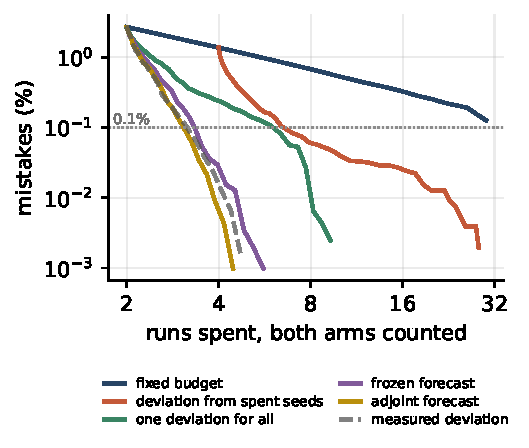
\includegraphics[width=\columnwidth]{sizing.pdf}
  \caption{Mistakes against runs spent. A policy is a curve, not a point, since the stopping
  threshold trades one against the other, and what separates two policies is how far left a curve
  sits at a fixed height. At $\numSizeTarget\%$ the forecasts cross near $\numSizeAdjointRuns$ runs
  and a fixed budget near $\numSizeFixedRuns$. The rule driven by spent seeds flattens on the left
  because it cannot stop before two seeds per arm however large the lead.}
  \label{fig:sizing}
\end{figure}

\subsection{Result}

The adjoint forecast reaches $\numSizeAdjointRuns$ runs and the ceiling, a rule handed the realised
deviation, reaches $\numSizeOracleRuns$: the same policy to within resampling error, at
$\numSizeOracleGain\times$ $[\numSizeOracleLo, \numSizeOracleHi]$. Fixed-budget practice needs
$\numSizeFixedRuns$ runs for the same reliability, $\numSizeFixedGain\times$
$[\numSizeFixedLo, \numSizeFixedHi]$ more. Estimating the deviation from spent seeds costs
$\numSizeEmpiricalGain\times$ $[\numSizeEmpiricalLo, \numSizeEmpiricalHi]$, and most of that is
structural rather than statistical: that rule cannot stop at one seed per arm however large the
lead, so four runs are committed before any comparison can be decided.

Grading against all $\numSizeSeeds$ seeds instead, so a policy's own seeds are part of the answer,
cuts the advantage over a fixed budget to $\numSizeOverlapFixed\times$. The overlap helps a policy
in proportion to how many seeds it draws, so it favours the baselines that draw the most, and the
headline numbers are the ones without it.

Note which predictor does the work. The frozen forecast \eqref{eq:frozen} uses the step size, the
run length and the two noise traces, with no stored trajectory and no backward pass. It reaches
$\numSizeFrozenRuns$ runs, within $\numSizeFrozenGain\times$ of the adjoint and still
$\numSizeFrozenVsFixed\times$ better than a fixed budget. The bulk of the saving does not require
Theorem~\ref{thm:adjoint} at all, and the backward pass buys the last $\numSizeFrozenGain\times$.
That is the cheap half a practitioner would deploy first.

\subsection{The other decision, where it helps less}

Sizing is not the only use of a deviation. The other is choosing: run each of several
configurations once and keep the one with the most gain per unit of noise and rollout. Reporting
only the decision that flatters the forecast would misrepresent it, so we measure both on the same
grid, with seeds split three ways and never reused across roles. One pilot supplies the observed
gain, a disjoint pool supplies whatever deviation a policy is entitled to, and a third reserved set
scores the choice. That last separation matters: letting the scoring seeds also set the deviation
makes an oracle look unbeatable, since its denominator then shares noise with the one it is graded
against, and an earlier version of this experiment did exactly that.

Over $\numPickTasks$ tasks the share of the best achievable value the choice keeps is
$\numPickConstant\%$ with one deviation for every recipe, $\numPickFrozen\%$ frozen,
$\numPickAdjoint\%$ adjoint and $\numPickOracle\%$ with the measured deviation: the forecast
recovers $\numPickGain$ points $[\numPickGainLo, \numPickGainHi]$ of the
$\numPickOraclePoints$ available, a share of $\numPickShare$.

The forecast is close to the ceiling in both decisions, but the ceilings differ. Choosing has only
$\numPickOraclePoints$ points of headroom at all, because a single pilot's observed gain is noisy
and that noise limits the choice whatever denominator is used. Sizing has no competing term: the
run count scales as $(\sigma/\mu)^2$, the deviation enters squared, and at one run per arm there is
no alternative estimate of it. That asymmetry, not the quality of the forecast, is why the two
numbers differ, and it is why we lead with sizing.

\subsection{How wrong the forecast may be}

On a pretrained model the forecast is accurate only in some regimes (Section~\ref{sec:real}), so we
corrupt it on purpose and rerun the benchmark: a lognormal multiplicative error of controlled
median magnitude, and separately a systematic scale error.

The scale error does nothing. Over $\numTolScaleRange$ orders of magnitude the runs needed change
by a factor of $\numTolScaleSpread$, because $z$ absorbs it exactly as \eqref{eq:stop} says. A
forecast used this way does not need to be calibrated, which is worth stating because it is the
opposite of what reporting an error bar requires.

Relative error is what costs. Runs needed rise from $\numTolClean$ at the measured accuracy to
$\numTolRunsOneHalf$ at a median error of $1.5\times$, $\numTolRunsDouble$ at $2\times$ and
$\numTolRunsTwoHalf$ at $2.5\times$, reaching the fixed budget's $\numTolFixed$ at about
$\numTolBreakeven\times$. The tolerance is wide but not unlimited: a forecast wrong by less than
roughly a factor of three pays for itself, and one wrong by twenty-five does not. That break-even
is the honest statement of scope, and Section~\ref{sec:real} is where it is tested.

\section{On pretrained models}
\label{sec:real}

Run end to end on Qwen2.5-0.5B with LoRA, the cheap estimator \eqref{eq:cheap} is a factor of
$\numRealShortCheap$ short of the measured spread and the transported one $\numRealShortTransported$. On Qwen2.5-7B under Adam,
with the recursion lifted to the optimiser state $z = (\theta, m, v)$, it is short by between
$\numAdamScaleShortfallLow$ and $\numAdamScaleShortfallHigh$. On the exact models the lift gives
$\numAdamLiftWarmMedian\times$ with Adam's moments warmed, but started cold and without bias
correction, as these runs were, its median error there is $\numAdamLiftColdRawMedian\times$ and
its worst $\numAdamLiftColdRawWorst\times$. Section~\ref{sec:forecast} reproduces the shortfall on exact
models once they learn, so it does not need a pretrained network.

\paragraph{Accuracy is regime-dependent, not uniformly poor.} On the corpus above the reward
groups go unanimous within five updates, yet its measured seed spread is the largest we report.
Most runs there learn to answer one constant: the stored run says ``1'' to every prompt, and
which constant a run falls into explains $\numModeSmallShare\%$ of the spread. So we built four corpora at
pre-specified mean live-group probabilities and ran the prospective test on each. The errors are
$\numSweepErrors$; the best, on the band at $\numSweepWinBand$, meets a criterion of $1.5\times$
declared before the sweep ran, forecasting $\numSweepWinForecast$ against a measured
$\numSweepWinMeasured$ $[\numSweepWinLow, \numSweepWinHigh]$ on a gain of $\numSweepWinGain$. So
local covariance forecasting can be quantitatively accurate on a pretrained model, though not
reliably so. Nor is collapse the cause: at $\numCollapseMissedBand$, where the forecast is
$\numCollapseMissedError\times$ too large, runs barely collapse, refuting two predictions we recorded beforehand.

All four sit inside the $\numTolLooseBreakeven\times$ break-even of Section~\ref{sec:sizing},
measured with $z$ read in sample; the unanimous corpus and $7$B under Adam do not.

\paragraph{The sizing benchmark at this scale.} Across $\numRealSizeRecipes$ recipes on one
corpus ($\numRealSizeRuns$ runs) the forecast holds up, at a median error of
$\numRealSizeError\times$ and a worst of $\numRealSizeErrorWorst\times$. The benchmark does not:
only $\numRealSizePairs$ of $\numRealSizeAllPairs$ pairs are ordered unambiguously at
$\numRealSizeMargin$ standard errors, most being genuine near-ties at sixteen seeds. On four
comparisons a stopping rule beats a fixed budget by $\numRealSizeFixedGain$
$[\numRealSizeFixedLo, \numRealSizeFixedHi]$ and nothing else separates. The
$\numSizeFixedGain\times$ of Section~\ref{sec:sizing} is therefore not demonstrated at this scale
and we do not claim it.

\paragraph{Two things the sweep falsified.} It does not support a monotone relationship between
stochastic support and accuracy: the ordering of errors across the four bands does not follow the
ordering of their live-group probabilities. And a one-run curvature diagnostic, calibrated on the
exact models to refuse forecasts whose runs are not small perturbations of each other, does not
transfer: it refuses every pretrained run, including the accurate one.

\section{Related work}
\label{sec:related}

\paragraph{Run-to-run variance.} That RL results move under reseeding is old news in deep RL
\citep{henderson2018matters} and documented again for language-model reasoning
\citep{hochlehnert2025sober}. Those papers establish the size of the problem by replication, which
is the only instrument available without a model of where the variance comes from.
\citet{agarwal2021precipice} prescribe how the resulting samples should be summarised. All of it
presumes the runs exist. Practice for benchmark error bars treats the evaluation set as the only
source of randomness \citep{miller2024adding}, which is the right interval for a fixed model and
the wrong one for a training procedure; \citet{bouthillier2021accounting} argue the pipeline's own
randomness belongs in the interval and estimate it by replication. We estimate the same quantity
without replicating, and our real-model measurements subtract the binomial term explicitly.

\paragraph{Deciding when to stop repeating.} Stopping a comparison once one arm is convincingly
ahead is sequential analysis \citep{wald1945sequential}, and its machine-learning form is racing
\citep{maron1993hoeffding, evendar2006action}, sharpened by using an empirical variance in the
bound \citep{audibert2009exploration} and scaled to hyperparameter search by allocating a budget
across candidates \citep{li2017hyperband}. Section~\ref{sec:sizing} uses the simplest rule of that
family deliberately: the contribution is not a better stopping rule but the quantity the rule
consumes. Every method there takes its variance from samples already drawn, which is sound when a
sample is a validation example and unaffordable when a sample is a training run. At one run per arm
those bounds are vacuous, and the experiment shows that the resulting floor, not the shape of the
bound, is what a comparison pays.

\paragraph{Stochastic dynamics of training.} Treating stochastic optimisation as a process whose
covariance is set by gradient noise against curvature is standard \citep{mandt2017sgd}, and
\eqref{eq:lyapunov} is not new as mathematics. What we add is the RLVR-specific measurement of
$Q_t$ through the two-level decomposition, the finite-time rather than stationary treatment, and
the observation that the filter, not the size of the noise, is what governs reproducibility here.
\citet{wang2026linear} reach a filtering picture from the opposite side, reporting near-linear
evolution of weights and log-probabilities; their object is one run's trajectory, ours the
covariance between runs differing only in seed.

\paragraph{Adjoint sensitivity.} Carrying a scalar backwards through a trajectory to avoid forming
a large intermediate is the adjoint method \citep{pontryagin1962mathematical, chen2018neural}.
Theorem~\ref{thm:adjoint} applies it to a covariance rather than a loss, and
Proposition~\ref{prop:potential} is what makes it cheap here by removing the transpose.

\paragraph{Entropy collapse.} That RLVR drives policy entropy down sharply is documented
\citep{cui2025entropy} and treated as an optimisation pathology. It has a second consequence that
follows from \eqref{eq:adjoint}: a count-based advantage is identically zero on a unanimous group,
so a collapsed policy injects $\Sigma_t = 0$, stops accumulating seed uncertainty, and any
measurement of its reproducibility from that point is measuring nothing.

\paragraph{Batch size and gradient noise.} The gradient noise scale predicts the batch size beyond
which data parallelism stops buying speed \citep{mccandlish2018empirical, shallue2019measuring}.
Both concern a single level of sampling. RLVR samples prompts and then responses within each
prompt, and the resulting two-level scale has no counterpart there; the decomposition itself is the
classical two-stage sampling result \citep{cochran1977sampling}.

\paragraph{Allocating rollouts.} Recent methods vary responses per prompt within a batch from pass
rates or gradient variance \citep{nguyen2026allocation}, or adapt batch size from a divergence
signal \citep{park2026batchscaling}. Those distribute responses \emph{within} one update, across
its prompts. The budget at issue here is across independent training runs of the same recipe, which
is a level those methods do not address and where the reproducibility cost is actually incurred.

\section{Limitations}
\label{sec:discussion}

\paragraph{The sizing benchmark.} The stopping rule \eqref{eq:stop} is not anytime-valid. Testing
after every seed and stopping on the first crossing inflates the error of a fixed-sample test, so
its nominal $z$ carries no coverage guarantee and we claim none. What we report is the mistake rate
the rule realises, measured against an ordering fixed on seeds no policy may draw. Every policy is
graded the same way and separated at a common realised rate, so the comparison does not rest on the
boundary being calibrated; a sequentially valid boundary would move all of them together, which we
expect but have not verified. Pairs whose ordering is ambiguous are excluded, so the benchmark says nothing about
near-ties, where the honest answer is to keep training whatever rule is in use.

\paragraph{Scale.} The largest model is a $4$-bit $7$B with $\numAdamScaleSeeds$ seeds, on one
laptop, and the exact tier where the forecast is validated is the furthest from a frontier run.

\paragraph{What the forecast costs.} Estimating the injected term from the eight prompts a run
trains on gives two forecasts $\numModeLargeRepeatRatio\times$ apart, because only about a tenth of
groups are not unanimous. Raising that to $\numAdamScaleWidePrompts$ prompts brings disjoint halves
to within $\numAdamScaleHalfRatio\times$ and costs $141$ minutes against the $260$ that training
all $\numAdamScaleSeeds$ seeds costs. A diagnostic consuming half the experiment it replaces is not
yet a diagnostic at this scale.

\paragraph{Claims we withdrew.} A predicted square-root relation between policy divergence and
outcome spread is not supported by our data. Nor is a short memory horizon: in $\numTiltedEarly$ of
$\numMemorySettings$ settings more of the final variance was injected in the first half of the run.
Token-level reshaping, length normalisation and clipping are outside \eqref{eq:family}.


\bibliography{../refs}

\end{document}
